% fig09_bstar_recurrence — B* = sigma*tau = 48 recurrence across 3 domains.
% Standalone pgfplots; compiled to figures/fig09_bstar_recurrence.pdf.
% Comparison (B* across RTSC/FUSION/UFO) => chart (user hard rule).
% Data: Appendix G, UFO/meta/cross-domain-mega.md §8.1 triple-SSOT.
%   RTSC Hc2 = 48 T, FUSION Lawson target = 48 T, UFO Meissner lift = 48 T.
%   Arithmetic-reuse OBSERVATION, not integrated-physics proof.
\documentclass[border=4pt]{standalone}
\usepackage{tikz}
\usepackage{pgfplots}
\pgfplotsset{compat=1.18}
\begin{document}
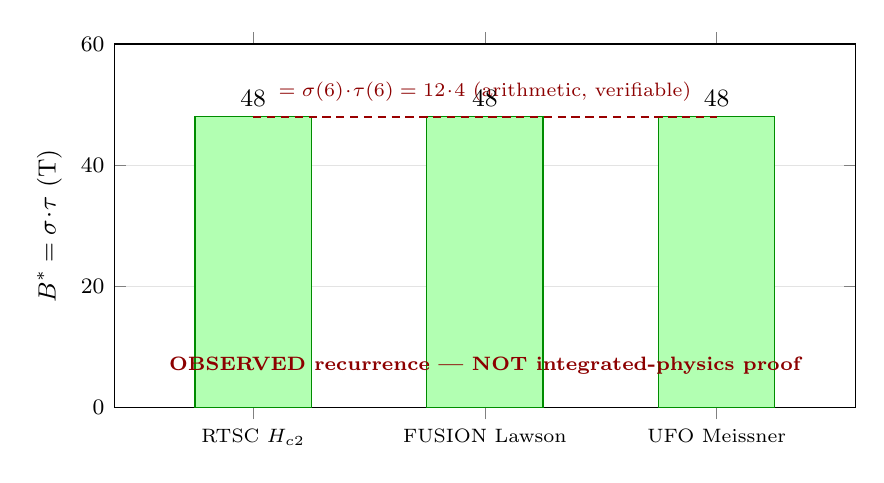
\begin{tikzpicture}
\begin{axis}[
  width=11cm, height=6.2cm,
  ybar,
  bar width=42pt,
  ymin=0, ymax=60,
  ylabel={$B^{*}=\sigma\!\cdot\!\tau$ (T)},
  symbolic x coords={{RTSC $H_{c2}$}, {FUSION Lawson}, {UFO Meissner}},
  xtick=data,
  x tick label style={font=\scriptsize},
  tick label style={font=\footnotesize},
  label style={font=\small},
  nodes near coords,
  nodes near coords style={font=\small},
  ymajorgrids, grid style={gray!22},
  enlarge x limits=0.30,
]
\addplot[draw=green!55!black,fill=green!30] coordinates {
  ({RTSC $H_{c2}$},48) ({FUSION Lawson},48) ({UFO Meissner},48)
};
\draw[red!60!black, thick, densely dashed] (axis cs:{RTSC $H_{c2}$},48) -- (axis cs:{UFO Meissner},48);
\node[red!55!black, font=\scriptsize, anchor=south] at (axis cs:{FUSION Lawson},49)
  {$=\sigma(6)\!\cdot\!\tau(6)=12\!\cdot\!4$ (arithmetic, verifiable)};
\node[red!55!black, font=\scriptsize\bfseries, anchor=north] at (axis cs:{FUSION Lawson},10)
  {OBSERVED recurrence --- NOT integrated-physics proof};
\end{axis}
\end{tikzpicture}
\end{document}
